\documentclass[iop]{emulateapj-rtx4}
%\documentclass[twocolumn,tighten]{aastex6}
%\documentclass{aastex6}
%\usepackage{emulateapj-rtx4}
%\usepackage{emulateapj}

 \shortauthors{French $\&$ Wakker}

\usepackage{graphicx}
\usepackage{subfigure}
\usepackage{hyperref}
\usepackage{amsmath}

%\usepackage{amssymb}
%\usepackage{wrapfig}
%\usepackage{setspace}

%\usepackage{mathtools}
%\frenchspacing

\newcommand{\kms}{$\rm km\, s^{-1}$}
\newcommand{\HI}{$H\,{\sc i}$}



\graphicspath{{figures//}}

\begin{document}

\title{Do Ly$\alpha$ absorbers co-rotate with galaxy disks?}

\author{David M. French, Bart P. Wakker}

\affil{Department of Astronomy, University of Wisconsin, Madison, WI 53706, USA}

\begin{abstract}

We present results of a study comparing the relative velocity of Ly$\alpha$ absorbers to the rotation direction and velocity of nearby galaxy disks. We find...

\end{abstract}


\keywords{galaxies:intergalactic medium, galaxies:evolution, galaxies:halos, quasars: absorption lines}


\section{INTRODUCTION}
Our current $\Lambda$CDM cosmology picture describes galaxies forming hierarchically out of overdensities in the underlying dark matter distribution. As matter is funneled toward a growing galaxy, conservation of angular momentum redistributes the angular momentum in this gas to match that of the halo and underlying dark matter as the gas is shock-heated and slowly cools. As this infalling gas is responsible for birthing and continuing to feed the galaxies, it is expected that the extended gaseous halos should rotate in the same sense as both the galactic disks and dark matter halos. Galaxy rotation curves have been observed to extend at constant velocity out to... (cite...). It becomes increasingly difficult to measure gas rotation much farther from this however as the density rapidly decreases. Within this region the galaxy disks transition into circumgalactic medium (CGM), and eventually the CGM merges with the intergalactic medium (IGM). At what point, however, does the surrounding medium cease to circulate with the galaxy? 

HYDRO? simulations such as those by Stewart et al. (2011, 2013) suggests that the bulk CGM kinematics out to (WHAT DISTANCE) may circulate, and that absorption in intervening QSO sightlines should be able to accurately capture this rotation signature. Observational confirmation, however, has be inconclusive. C\^{o}t\'{e} et al. 2005 probed the halos of nine galaxies using \emph{HST} observed background QSOs, finding large warps would be needed to explain the velocity of \HI~absorbers by an extended rotating disk. Wakker \& Savage (2009) compiled a sample of 4 galaxy-QSO systems from the literature, finding only 1/4 of Ly$\alpha$ absorbers appeared to co-rotate with the associated galaxy disk. Approaching the question from a different angle, Bowen et al. (2016) probed the halo of a single galaxy, NGC1097, with 4 nearby QSO sightlines, and suggests that an extended, slowly rotating disk with additional inflowing IGM material best matches observations.

%There have been several studies with a sample size of one or a few aiming to compare the kinematics of the galaxy disk to absorption detected in it's CGM halo (e.g., C\^{o}t\'{e} et al. 2005; Wakker \& Savage 2009; Bowen et al. 2016; \textbf{MORE}). With these individual results we may be missing the forest for the sake of the individual trees. There has yet to be a more systematic search for observational evidence that the CGM is kinematically associated with galaxies in general.

Numerous studies have shown a correlation between equivalent width and decreasing velocity difference between galaxies and IGM absorbers (e.g., French \& Wakker 2017, MORE).

To make progress here, we have obtained rotation curves for 12 nearby spiral galaxies which are located within 500 kpc of a background QSO observed by the Cosmic Origins Spectrograph (COS) on \textit{HST}. 

We have augmented this new sample with additional galaxies with known rotation velocity and orientation from the literature. In Section 2 we describe the selection and reduction of both SALT and COS spectra. We then discuss each galaxy-QSO system in detail in Section 3, and introduce our halo-velocity model for interpreting these systems in Section 4. In Section 5 we discuss the overall results of this exercise and present a physically-motivated interpretation of these results. See Section 6 for a summary of our results and conclusions.




\begin{table*}[ht]\footnotesize
\begin{center}
\begin{tabular}{l l l l l l l l l l c}
 \hline \hline
  Target 					& Galaxy				& R.A. 				& Dec. 				& \textit{z}		& Program 	 & Grating 	  & Obs ID 	    & Obs Date		& $T_{exp}*$	& S/N*  \\ 
  	    					& 	       				&	  				& 		  	 		& 		    	& 		  	 & 		  	   & 		     	    & 				& [ks]		& [1238] \\ 
 \scriptsize (1)  				& \scriptsize (2) 		& \scriptsize (3) 		& \scriptsize (4) 		& \scriptsize (5) & \scriptsize (6) & \scriptsize  (7) & \scriptsize (8) & \scriptsize (9) 	& \scriptsize (10) & \scriptsize (11)  \\ \hline \hline
\\
%1H0717+714		  							&  	07  21  53.3  		&     +71  20  36.0  	&    0.5003  	& 12025  		&   G130M  	&   LBG812  	& 11-12-27  &  6.0    &      37         \\
1H0419-577  				&      NGC1566  		&      04  26  00.7  		&	-57  12  02.0  	&   0.10400  	& 11686		&   G130M	&   Obs ID  & Obs Date  & 20429  &      75         \\
1H0419-577  				&      NGC1566  		&      04  26  00.7  		&	-57  12  02.0  	&   0.10400  	& 11686		&   G160M	&   Obs ID  & Obs Date  & 15934  &      55         \\
HE0429-5343  				&      NGC1566  		&      04  30  40.0  		&	-53  36  56.0 	&   0.04001  	& 12275		&   G130M	&   Obs ID  & Obs Date  & 2067  &       12         \\
HE0435-5304  				&      NGC1566  		&      04  36  50.9  		&      -52  58  47.0  	&   0.42616  	& 11520		&   G130M	&   Obs ID  & Obs Date  & 8372  &       12         \\
HE0435-5304  				&      NGC1566  		&      04  36  50.9  		&	-52  58  47.0  	&   0.42616  	& 11520		&   G160M	&   Obs ID  & Obs Date  & 8935  &       9           \\
%HE0435-5304  			&      NGC1566  		&      04  36  50.9  		&	-52  58  47.0  	&   0.42616  	& 11520		&   G285M	&   Obs ID  & Obs Date  & 4286  &       2           \\
RBS567  					&      NGC1566  		&      04  39  38.7  		&	-53  11  31.0  	&   0.24300  	& 11520		&   G130M	&   Obs ID  & Obs Date  & 8176  &       17         \\
RBS567  					&      NGC1566  		&      04  39  38.7  		&	-53  11  31.0  	&   0.24300  	& 11520		&   G160M	&   Obs ID  & Obs Date  & 8933  &       11         \\
%RBS567  				&      NGC1566  		&      04  39  38.7  		&	-53  11  31.0  	&   0.24300  	& 11520		&   G285M	&   Obs ID  & Obs Date  & 4286  &       2           \\
HE0439-5254  				&      NGC1566  		&      04  40  12.0  		&	-52  48  18.0  	&   1.05300  	& 11520		&   G130M	&   Obs ID  & Obs Date  & 8402  &       18         \\
HE0439-5254				&      NGC1566  		&      04  40  12.0  		&	-52  48  18.0  	&   1.05300  	& 11520		&   G160M	&   Obs ID  & Obs Date  & 8935  &       13         \\
%HE0439-5254 			&      NGC1566  		&      04  40  12.0  		&	-52  48  18.0  	&   1.05300  	& 11520		&   G285M	&   Obs ID  & Obs Date  & 4316  &       2           \\
H1101-232  				&      NGC3513  		&      11  03  37.7  		&	-23  29  31.0  	&   0.18600  	& 12025		&   G130M	&   Obs ID  & Obs Date  & 13341  &      16         \\
H1101-232  				&      NGC3513  		&      11  03  37.7  		&	-23  29  31.0  	&   0.18600  	& 12025		&   G160M	&   Obs ID  & Obs Date  & 13296  &      10         \\
SDSSJ112005.00+041323.0  	& 	NGC3633  		&      11  20  05.0  		&	+04  13  23.0 	&   0.54689  	& 12603		&   G130M	&   Obs ID  & Obs Date  & 4708  &       9            \\
RX\_J1121.2+0326  			&      CGCG039-137 		&   	11  21  14.0  		&	+03  25  47.0 	&   0.15200  	& 12248		&   G130M	&   Obs ID  & Obs Date  & 2695  &       5           \\
RX\_J1121.2+0326  			&      NGC3633  		&	11  21  14.0  		&	+03  25  47.0 	&   0.15200  	& 12248		&   G130M	&   Obs ID  & Obs Date  & 2695  &       5          \\
RX\_J1121.2+0326  			&      CGCG039-137 		&	11  21  14.0  		&	+03  25  47.0 	&   0.15200  	& 12248		&   G160M	&   Obs ID  & Obs Date  & 4741  &       4           \\
RX\_J1121.2+0326  			&      NGC3633  		&      11  21  14.0  		&	+03  25  47.0 	&   0.15200  	& 12248		&   G160M	&   Obs ID  & Obs Date  & 4741  &       4           \\
SDSSJ112224.10+031802.0  	& 	CGCG039-137 		&  	11  22  24.1  		&	+03  18  02.0 	&   0.47528  	& 12603		&   G130M	&   Obs ID  & Obs Date  & 7588  &       10          \\
3C273.0  					&	NGC4536  		&      12  29  06.7  		&	+02  03  09.0 	&   0.15834  	& 12038		&   G130M	&   Obs ID  & Obs Date  & 4002  &       111         \\
%3C273.0  				&      NGC4536  		&      12  29  06.7  		&	+02  03  09.0 	&   0.15834  	& 1029		&   G130H		&   Obs ID  & Obs Date  & 10480  &      0            \\
%3C273.0  				&      NGC4536  		&      12  29  06.7  		&	+02  03  09.0 	&   0.15834  	& 1029		&   G190H		&   Obs ID  & Obs Date  & 2880  &       0            \\
%3C273.0  				&      NGC4536  		&      12  29  06.7  		&	+02  03  09.0 	&   0.15834  	& 1029		&   G270H		&   Obs ID  & Obs Date  & 1440  &       0            \\
%3C273.0  				&      NGC4536  		&      12  29  06.7  		&	+02  03  09.0  	&   0.15834  	& 3088		&   G190H		&   Obs ID  & Obs Date  & 5416  &       0            \\
%3C273.0  				&      NGC4536  		&      12  29  06.7  		& 	+02  03  09.0  	&   0.15834  	& 3088		&   G270H		&   Obs ID  & Obs Date  & 5416  &       0            \\
3C273.0  					&      NGC4536  		&      12  29  06.7  		&	+02  03  09.0 	&   0.15834  	& 1140		&   G160M	&   Obs ID  & Obs Date  & 30028  &      55         \\
%3C273.0  				&      NGC4536  		&      12  29  06.7  		& 	+02  03  09.0  	&   0.15834  	& 1140		&   G200M	&   Obs ID  & Obs Date  & 979  &        10           \\
%3C273.0  				&      NGC4536  		&      12  29  06.7  		&	+02  03  09.0  	&   0.15834  	& 1140		&   G270M	&   Obs ID  & Obs Date  & 1958  &       14          \\
%3C273.0  				&      NGC4536  		&      12  29  06.7  		&	+02  03  09.0  	&   0.15834  	& 8017		&   E140M		&   Obs ID  & Obs Date  & 18671  &      23         \\
HE1228+0131  				&      NGC4536  		&      12  30  50.0  		&	+01  15  23.0  	&   0.11700  	& 11686		&   G130M 	&   Obs ID  & Obs Date  & 11036  &      61          \\
HE1228+0131  				&      NGC4536  		&      12  30  50.0  		&	+01  15  23.0  	&   0.11700  	& 11686		&   G160M	&   Obs ID  & Obs Date  & 11029  &      45          \\
%HE1228+0131  			&      NGC4536  		&      12  30  50.0  		&	+01  15  23.0  	&   0.11700  	& 6410		&   G160M	&   Obs ID  & Obs Date  & 11750  &      10           \\
%HE1228+0131  			&      NGC4536  		&      12  30  50.0  		&	+01  15  23.0  	&   0.11700  	& 7737		&   E140M		&   Obs ID  & Obs Date  & 27228  &      9            \\
LBQS1230-0015  			&      NGC4536  		&      12  33  04.1  		&	-00  31  34.0  	&   0.47095  	& 11598		&   G130M	&   Obs ID  & Obs Date  & 10323  &      13          \\
LBQS1230-0015  			&      NGC4536  		&      12  33  04.1  		&	-00  31  34.0  	&   0.47095  	& 11598		&   G160M	&   Obs ID  & Obs Date  & 5896  &       7            \\
%PG1302-102  			&      NGC4939  		&      13  05  33.0  		&	-10  33  20.0  	&   0.27840  	& 8306		&   E140M		&   Obs ID  & Obs Date  & 22119  &      7            \\
PG1302-102  				&      NGC4939  		&      13  05  33.0  		&	-10  33  19.0  	&   0.27840  	& 12038		&   G130M	&   Obs ID  & Obs Date  & 5979  &       27          \\
PG1302-102  				&      NGC4939  		&      13  05  33.0  		&	-10  33  19.0  	&   0.27840  	& 12038		&   G160M	&   Obs ID  & Obs Date  & 6867  &       34          \\
%PG1302-102  			&      NGC4939  		&	13  05  33.0  		&	-10  33  19.0  	&   0.27840  	& 3791		&   G130H		&   Obs ID  & Obs Date  & 18530  &      0            \\
%PG1302-102  			&      NGC4939  		&      13  05  33.0  		&	-10  33  19.0  	&   0.27840  	& 3222		&   G190H		&   Obs ID  & Obs Date  & 2442  &       0           \\
%PG1302-102  			&      NGC4939  		&      13  05  33.0  		&	-10  33  19.0  	&   0.27840  	& 3222		&   G270H		&   Obs ID  & Obs Date  & 939  &        0            \\
SDSSJ135726.27+043541.4  	&	NGC5364  		&      13  57  26.3  		&	+04  35  41.0  	&   1.23453  	& 12264		&   G130M	&   Obs ID  & Obs Date  & 14148  &      15           \\
SDSSJ135726.27+043541.4  	& 	NGC5364  		&      13  57  26.3  		&	+04  35  41.0  	&   1.23453  	& 12264		&   G160M	&   Obs ID  & Obs Date  & 28206  &      12          \\
QSO1500-4140  			&      NGC5786  		&      15  03  34.0  		&	-41  52  23.0  	&   0.33500  	& 11659		&   G130M	&   Obs ID  & Obs Date  & 9258  &       9           \\
SDSSJ151237.15+012846.0  	& 	UGC09760  		&      15  12  37.2  		&	+01  28  46.0  	&   0.26625  	& 12603		&   G130M	&   Obs ID  & Obs Date  & 7590  &       6           \\
RBS1768  				&      ESO343-G014  	&   	21  38  49.9  		&	-38  28  40.0  	&   0.18299  	& 12936		&   G130M	&   Obs ID  & Obs Date  & 6962  &       24          \\
RBS1768  				&      ESO343-G014  	&	21  38  49.9  		&	-38  28  40.0  	&   0.18299  	& 12936		&   G160M	&   Obs ID  & Obs Date  & 3837  &       11           \\
MRC2251-178  			&      MCG-03-58-009  	& 	22  54  05.9  		&	-17  34  55.0  	&   0.06609  	& 12029		&   G130M	&   Obs ID  & Obs Date  & 5515  &       42           \\
MRC2251-178  			&      MCG-03-58-009  	& 	22  54  05.9  		&	-17  34  55.0  	&   0.06609  	& 12029		&   G160M	&   Obs ID  & Obs Date  & 7125  &       30           \\
%MRC2251-178  			&      MCG-03-58-009  	& 	22  54  05.9  		&	-17  34  55.0  	&   0.06609  	& 6484		&   G130H		&   Obs ID  & Obs Date  & 4740  &       0           \\
%MRC2251-178  			&      MCG-03-58-009  	& 	22  54  05.9  		&	-17  34  55.0  	&   0.06609  	& 6484		&   G190H		&   Obs ID  & Obs Date  & 1730  &       0            \\
%MRC2251-178  			&      MCG-03-58-009  	& 	22  54  05.9  		&	-17  34  55.0  	&   0.06609  	& 6484		&   G270H		&   Obs ID  & Obs Date  & 300  &        0            \\
%MRC2251-178  			&      MCG-03-58-009  	& 	22  54  05.9  		&	-17  34  55.0  	&   0.06609  	& 7345		&   G140M	&   Obs ID  & Obs Date  & 10574  &      32           \\
RBS2000  				&      IC5325  			&      23  24  44.7  		&	-40  40  49.0  	&   0.17359  	& 13448		&   G130M	&   Obs ID  & Obs Date  & 5046  &       18           \\
RBS2000  				&      IC5325  			&      23  24  44.7  		&	-40  40  49.0  	&   0.17359  	& 13448		&   G160M	&   Obs ID  & Obs Date  & 5726  &       12           \\

 \\
\hline

\end{tabular}
\end{center}
  \caption{\small{COS targets in this sample. *Total exposure time and S/N ratio is given for multi-orbit exposures.}}
  \label{target_table}
\end{table*}


\section{DATA AND ANALYSIS}

\subsection{SALT Data}
Our sample contains 12 galaxies observed with the Southern African Large Telescope (SALT) Robert Stobie Spectrograph (RSS) in longslit mode. These 12 were selected from a larger pool of 48 submitted targets by the SALT observing queue. These 48 possible targets were chosen for their proximity to background QSOs whose spectra contained promising Ly$\alpha$ lines. Finally, we only included galaxies with $z \leq 0.33$ ($cz \leq 10,000$ \kms), angular sizes less than 6' to enable easy sky subtraction without taking additional exposures, and surface brightnesses sufficient to keep exposure times below $\sim 1300 s$. Table \ref{salt_targets} summarizes these observations. Data was taken for 2 additional galaxies, NGC3640 and NGC2962, but proved unusable due to issues with spectral identification and low signal-to-noise (respectively).

%All SALT galaxy spectra were reduced and extracted using the standard PySALT reduction package (\textbf{\begin{table*}[ht]\footnotesize. 


All SALT galaxy spectra were reduced and extracted using the standard PySALT reduction package (\textbf{CITATION}), which includes procedures to prepare the data, correct for gain, cross-talk, bias, and overscan, and finally mosaic the images from the 3 CCDs. Next, we rectify the images with wavelength solutions found via Ne and Ar arc lamp spectra line identification. Finally, we perform a basic sky subtraction using an off-sky portion of the spectrum, and extract 5-10 pixel wide 1-D strips from the reduced 2-D spectrum. 

For each 1-D spectrum, we identify the H$\alpha$ emission lines and perform a non-linear least-squares Voigt profile fit using the Python package LMFIT\footnote{\url{http://cars9.uchicago.edu/software/python/lmfit/contents.html}}. The line centroid and 1$\sigma$ standard errors are returned, and these fits are then shifted to rest-velocity based on the galaxy systemic redshift and heliocentric velocity corrections are calculated with the IRAF rvcorrect procedure. The final rotation velocity is calculated by then applying the inclination correction, $v_{rot} = v / \sin(i)$. Final errors are calculated as a quadrature sum of $1\sigma$ fit errors, systemic redshift error, and inclination uncertainty as follows:

\begin{equation}
\begin{split}
	\sigma^2 = \left( \frac{\partial v_{rot}}{\partial \lambda_{obs}} \right)^2 (\Delta \lambda_{obs})^2 + \left(\frac{\partial v_{rot}}{\partial v_{sys}} \right)^2 (\Delta v_{sys})^2 + \\
	\left( \frac{\partial v_{rot}}{\partial i} \right)^2 (\Delta i)^2,
\end{split}
\end{equation}

\noindent where $\Delta \lambda_{obs}$, $\Delta v_{sys}$, and $\Delta i$ are the errors in observed line center, galaxy redshift, and inclination, respectively. 

We determine the inclination error by calculating the standard deviation of the set of all axis ratio values available in NED for each galaxy. The final physical scale is calculated using the SALT image scale of 0.1267 arcsec/pixel, multiplied by the 4-pixel spatial binning, and converted to physical units using a redshift-independent distance if available, and a Hubble flow estimate if not. We adopt a Hubble constant of $H_0$ = 71 \kms $\rm Mpc^{-1}$ throughout.

Finally, we calculate our approaching and receding velocities via a weighted mean of the outer 1/2 of each rotation curve, with errors calculated as weighted standard errors in the mean. Our final redshifts are calculated by forcing symmetric rotation, such that the outer 1/2 average velocity for each side matches in magnitude. See Figure \ref{rotationcurve} for an example.

%\begin{figure}[b!]
%        \centering
%        \vspace{0pt}
%        \includegraphics[width=0.50\textwidth]{NGC3633_2_rotation_curve_xphys_helio_vobs_vrotObs_new4.pdf}
%        \caption{\small{Rotation curve of NGC3633. The solid green line indicates the weighted mean velocity over the corresponding x-axis region, and the shaded green indicates the 1$\sigma$ error in the mean.}}
%        \label{completeness}
%\end{figure}

\begin{figure}[t!]
\centering
  \subfigure[]{\includegraphics[width=1.\linewidth]{NGC3633_2_rotation_curve_xphys_helio_vobs_vrotObs_new4.pdf}}{\label{rotationcurve}}
  \subfigure[]{\includegraphics[width=0.95\linewidth]{NGC3633_FindingChart.pdf}\label{finderchart}}
  \caption{\small{a) Rotation curve of NGC3633. The solid green line indicates the weighted mean velocity over the corresponding x-axis region, and the shaded green indicates the 1$\sigma$ error in the mean. b) SALT finder chart for NGC3633 showing the position of the slit in red.}}
\vspace{5pt}
\end{figure}




\begin{table*}[ht]\footnotesize. 
\begin{center}
\begin{tabular}{l l l l l l l l l l}
 \hline \hline
%  Galaxy 		 	& R.A. 			& Dec. 		 	& \textit{cz}		& Type		& Grating		& LOS Velocity		& Inc. Corrected Velocity	& Obs Date	& $T_{exp}$		\\ 
  Galaxy 		 	& R.A. 			& Dec. 		 	& \textit{cz}		& Type		& Grating		& $\rm V_{rot}$		& $\rm V_{rot} / \sin(\emph{i})$	& Obs Date	& $T_{exp}$		\\ 

  	    		 	& 	       			&	  		 	& (\kms)			& 		  	&			& [\kms]		     	& [\kms]				&			& [ks]			\\ 
 \scriptsize (1)  	 	& \scriptsize (2)		& \scriptsize (3) 	& \scriptsize (4)		& \scriptsize (5)	& \scriptsize (6)	& \scriptsize (7)		& \scriptsize (8)			& \scriptsize (9)	& \scriptsize (10)	\\ \hline \hline
 
 CGCG039-137 	& 11 21 26.95		& +03 26 41.68		& $6918 \pm24$	& Scd		& PG2300		& $132 \pm 16$	& $139 \pm 26$		& 05 11 2016	& 700			\\ %done
 
 IC5325		 	& 23 28 43.43		& $-$41 20 0.49	& $1512 \pm8$		& SAB(rs)bc	& PG2300		& $53 \pm 5$		& $125 \pm 39$		& 05 17 2016	& 600			\\ %done
 
 MCG-03-58-009	& 22 53 40.85		& $-$17 28 44.00	& $9015 \pm19$	& Sc			& PG2300		& $150 \pm 12$	& $171 \pm 23$		& 05 16 2016	& 1200			\\ %done

 NGC1566		& 04 20 0.42		& $-$54 56 16.12	& $1502 \pm15$	& SAB(rs)bc	& PG2300		& $64 \pm 8$		& $195 \pm 47$		& 10 18 2016	& 400			\\ %done

 NGC3513		& 11 03 46.08		& $-$23 14 43.8	& $1204 \pm12$	& SB(s)c		& PG2300		& $11 \pm 10$		& $22 \pm 24$			& 05 26 2016	& 600			\\ %done
 
 NGC3633	 	& 11 20 26.22		& +03 35 8.20		& $2587 \pm7$		& SAa		& PG2300		& $149 \pm 6$		& $157 \pm 9$			& 05 11 2016	& 1200			\\ %done

 NGC4536	 	& 12 34 27.05		& +02 11 17.30		& $1867 \pm33$	& SAB(rc)bc	& PG2300		& $129 \pm 9$		& $148 \pm 41$		& 05 11 2016	& 1300			\\ %done

 NGC4939		& 13 04 14.39		& $-$10 20 22.60	& $3093 \pm33$	& SA(s)bc		& PG2300		& $204 \pm 25$	& $275 \pm 66$		& 05 14 2016	& 500			\\ %done

 NGC5364	 	& 13 56 12.00		& +05 00 52.09		& $1238 \pm17$	& SA(rs)bc pec	& PG2300		& $130 \pm 13$	& $155 \pm 22$		& 05 11 2016	& 700			\\ %done
 
 NGC5786	 	& 14 58 56.26		& $-$42 00 48.10	& $2975 \pm22$	& SAB(s)bc	& PG2300		& $156 \pm 10$	& $172 \pm 25$		& 05 11 2016	& 250			\\ %done

 RFGC3781	 	& 21 37 45.18		& $-$38 29 33.22	& $9139 \pm32$	& S			& PG2300		& $203 \pm 32$	& $203 \pm 32$		& 05 16 2016	& 1000			\\ %done

 UGC09760	 	& 15 12 02.44		& +01 41 55.46		& $2094 \pm16$	& Sd			& PG2300		& $46 \pm 10$		& $46 \pm 16$			& 05 11 2016	& 500			\\


 \hline

\end{tabular}
\end{center}
  \caption{\small{SALT targeted galaxies. Columns are as follows: 1) the galaxy name, 2), 3) R.A., Dec. in J2000, 4) galaxy systemic velocity, 5) morphological type (RC3), 6) RSS grating used, 7) approaching side velocity, 8) receding side velocity, 9) observation date, 10) exposure time, and 11) S/N of the H$\alpha$ or Ca H\&K lines.}}
  \label{salt_targets}
\end{table*}

\subsection{COS Spectra}
The Barbara A. Mikulski Archive for Space Telescopes (MAST) archives yield 19 QSO targets observed by COS which lie within 500 kpc of our SALT galaxies. These targets vary widely in signal-to-noise from approximately 5 to 100 due to our choosing them based only on their proximity to galaxies with known rotation. The reduction procedure for these spectra follow those described by French $\&$ Wakker 2017 and Wakker et al. (2015). In short, spectra are processed with CALCOS vXXXX? and combined via the method of Wakker et al. (2015), which helps corrects the COS wavelength scale misalignments produced by CALCOS. Multiple exposures are combined via alignment with Galactic 21cm absorption spectra and summing total counts per pixel before converting to flux. The COS instrument is described in detail by Green et al. (2012).


\section{SALT Galaxies}

\subsection{CGCG039-137}

CGCG039-137 is an isolated Scd type galaxy with a measured systemic velocity of $6918 \pm 24$ \kms~and inclination of $63^{\circ}$. There are two associated sightlines: RX\_J1121.2+0326 at an impact parameter of 99 kpc and azimuth angle of $71^{\circ}$ on the receding side, and SDSSJ112224.10+031802.0 at 491 kpc and $24^{\circ}$ on the approaching side. Ly$\alpha$ absorption is detected in both sightlines within $400$\kms~ of CGCG039-137. 

Towards RX\_J1121.2+0326 we detect Ly$\alpha$ at 6975 \kms~, which, at $\Delta v = 57$ \kms, lies well within the range of projected velocities consistent with co-rotation. The absorber detected toward SDSSJ112224.10+031802.0 occurs at a more distant 6606 \kms ($\Delta v = -312$ \kms). Although this absorber has the correct sign for co-rotation (blue-ward on the approaching side of the disk), the large velocity difference and impact parameter make it unlikely that this absorption can be linked to coherent halo rotation.


%Systemic velocity as published: 6902
%Velocity as measured: 6917.8 $\pm$ 23.7
%Rotation velocity (inc corrected) 139 $\pm$ 26 \kms
%Rotation velocity (observed) 132 $\pm$ 16 \kms
%Inclination: 61
%Adjusted Inc: 63
%Morphology: Scd
%$L_{\**}$ = 0.62 \\
%
%Two sightlines: \\
%RX\_J1121.2+0326 at 99 kpc, 71deg az: \\
%6975 Lya (dv = 75 \kms on pos side)
%
%SDSSJ112224.10+031802.0 at 491 kpc, 24deg az : \\
%6606 Unmarked (dv = -312 \kms on neg side)


\subsection{ESO343-G014}
ESO343-G014 is an edge on spiral galaxy with a measured systemic velocity of 9138.9 $\pm$ 31.7 \kms. It has a smaller neighboring galaxy, 2MASXJ21372816-3824412, located north of it's major axis at a projected distance of 216 kpc and velocity of 9129. The nearest sightline is towards RBS1768 at an impact parameter of 466kpc and $74^{\circ}$ azimuth angle on the approaching side. We detect 3 Ly$\alpha$ absorption lines within 300 \kms of ESO343-G014 (at 9308, 9360, and 9434 \kms). All of these are anti-aligned with the rotation of ESO343-G014, but unfortunately the presence of 2MASXJ21372816-3824412 makes it difficult to attribute this gas solely to ESO343-G014. Additionally, this gas could be attributed to either the approaching or receding side of the disk due to the large impact parameter and high azimuth angle of the sightline.


%Systemic velocity as published: 9162
%Velocity as measured: 9138.9 $\pm$ 31.7
%Rotation velocity (inc corrected) 205 $\pm$ 53 \kms
%Rotation velocity (observed) 203 $\pm$ 6 \kms
%Inclination: 84
%Adjusted Inc: 90
%Morphology: Sb
%$L_{\**}$ = 1.1 \\
%
%One sightline: \\
%RBS1768 at 466 kpc, 74deg az: \\
%9308 Lya (dv = 169 \kms on pos side)
%9360 Lya (dv = 221 \kms on pos side)
%9434 Lya (dv = 295 \kms on pos side)


\subsection{IC5325}
IC5325 is a face-on SAB(rs)bc type galaxy with a measured velocity of 1511.9 $\pm$ 8.4 \kms. It's inclination is just high enough ($25^{\circ}$) to obtain a reasonable rotation curve. The closest neighboring galaxy is ESO347-G020 to the Southeast at 306 kpc and a heliocentric velocity of 1745 \kms. Three other much smaller galaxies are also located $\sim 450$ kpc to the Southwest. We detect Ly$\alpha$ absorption at 1598\kms, $\Delta v = 86$\kms~in the spectrum towards RBS2000 at an impact parameter of 314 kpc and azimuth angle of $64^{\circ}$ on the approaching side. While this velocity is anti-aligned with the rotation the disk gas, the low inclination angle of IC5325 leads to a highly uncertain position angle. Without additional observations, we cannot say for certain if the location of RBS2000 actually lies on the approaching or receding side. This position angle uncertainty also means our SALT rotation curve is a lower limit on the true rotation velocity of IC5325.

%The velocity of the absorber, $\Delta v = 86$\kms, is also outside the range of projected co-rotation velocities


% Two galaxies are neighboring IC5325 to the South and East: PGC071660 at XXX kpc and NGC7552 at XXX kpc. 
 

%Systemic velocity as published: 1503
%Velocity as measured: 1511.9 $\pm$ 8.4
%Rotation velocity (inc corrected) 125 $\pm$ 45 \kms
%Rotation velocity (observed) 53 $\pm$ 5 \kms
%Inclination: 25
%Adjusted Inc: 25
%Morphology: SAB(rs)bc
%$L_{\**}$ = 0.9 \\
%
%One sightline: \\
%RBS2000 at 314 kpc, 64deg az: \\
%1598 Lya (dv = 86 \kms on possibly? neg side)


\subsection{MCG-03-58-009}
MCG-03-58-009 is a massive and very isolated Sc type galaxy at a measured velocity of $9015 \pm 19$ \kms~ and inclination angle of $49^{\circ}$. A weak Ly$\alpha$ absorber is detected at $9029$ \kms~towards MRC2251-178, which lies 355 kpc away at an azimuth angle of $71^{\circ}$ on the receding side. Although this absorber matches the velocity direction expected for co-rotation, the velocity difference ($\Delta v = 14$ \kms) is within the systemic velocity uncertainty. The relative weakness of this absorber (EW = $62 \pm 4$ m\AA) is somewhat surprising given it's proximity (just outside of 1 $R_{vir}$) to a massive galaxy. If this is representative of an isolated system such as MCG-03-58-009, then we should expect the halo rotational velocity to approach systemic by 1 $R_{vir}$.

%Systemic velocity as published: 9030
%Velocity as measured: 9014.9 $\pm$ 18.6
%Rotation velocity (inc corrected) 171 $\pm$ 24 \kms
%Rotation velocity (observed) 150 $\pm$ 12 \kms
%Inclination: 48
%Adjusted Inc: 49
%Morphology: Sc
%$L_{\**}$ = 2.9 \\
%
%One sightline: \\
%MRC2251-178 at 355 kpc, 71deg az: \\
%9029 Lya (dv = 14 \kms on pos side)



\subsection{NGC1566}
NGC1566 is well sampled (5 nearby QSO sightlines), but unfortunately also part of a complex environment of neighboring galaxies. We detect Ly$\alpha$ in all 5 of these sightlines. The farthest three, HE0439-5254, RBS567, and HE0435-5304, are clustered close together to the northeast of NGC1566 at $\gtrsim 395$ kpc and azimuth angles of $\sim 60^{\circ}$. 

HE0429-5343 is in the same direction and azimuth angle but closer at $\rho = 256$ kpc, and shows Ly$\alpha$ absorption at 1167 and 1358 \kms. These absorbers both have the correct velocity \emph{sign}, but we would expect a smaller velocity for co-rotation (approximately $\Delta v \sim \pm40$ \kms~projected). This difference could be explained by invoking either a warped extended disk, or perhaps inflowing gas.

1H0419-577 is located to the south at 303 kpc and just east of the receding side of the major axis at an azimuth angle of $10^{\circ}$. We detect Ly$\alpha$ at 1071, 1123, 1188, 1264, and 2020 \kms, all of which are the wrong sign for co-rotation or distant in velocity. This sightline is actually closer to a small group of galaxies including NGC1549, NGC1546 and NGC1536, all with systemic velocities near $1200$ \kms. We expect the lines at 1071, 1123, 1188, 1264 \kms~to be associated with this group rather than with NGC1566.

%Systemic velocity as published: 1504
%Velocity as measured: 1501.9 $\pm$ 14.9
%Rotation velocity (inc corrected) 86 $\pm$ 21 \kms
%Rotation velocity (observed) 64 $\pm$ 13 \kms
%Inclination: 46
%Adjusted Inc: 48
%Morphology: (R'\_1)SAB(rs)bcSy1
%$L_{\**}$ = 0.59
%Five sightlines: 

% south
%1H0419-577 at 303 kpc, 10deg az: \\
%1071 Lya (dv = -427 \kms on pos side) EW = 249 \pm 2
%1123 Lya (dv = -379 \kms on pos side) EW = 269 \pm 1
%1188 Lya (dv = -314 \kms on pos side) EW = 240 \pm 1
%1264 Lya (dv = -238 \kms on pos side) EW = 91 \pm 2
%2020 Lya (dv = 518 \kms on pos side) EW = 9 \pm 1
%
%% northeast close
%HE0429-5343 at 256 kpc, 60deg az: \\
%1167 Lya (dv = -335 \kms on neg side) EW = 79 \pm 14
%1358 Lya (dv = -144 \kms on neg side) EW = 136 \pm 21
%
%
%% northeast far
%HE0435-5304 at 396 kpc, 62deg az: \\
%1512 Lya (dv = 12 \kms on neg side) EW = 220 \pm 12
%1633 Lya (dv = 131 \kms on neg side) EW = 217 \pm 10
%1690 Lya (dv = 188 \kms on neg side) EW = 204 \pm 11
%
%RBS567 at 423 kpc, 69deg az: \\
%1664 Lya (dv = 162 \kms on neg side) EW = 517 \pm 10
%
%HE0439-5254 at 459 kpc, 65deg az: \\
%1148 Lya (dv = -354 \kms on neg side) EW = 72 \pm 11
%1649 Lya (dv = 147 \kms on neg side) EW = 501 \pm 9



\subsection{NGC3513}
NGC3513 a mostly face-on SB(rs)c galaxy with heliocentric velocity $V_{hel} = 1204 \pm 12$ \kms. It has a companion galaxy in NGC3511 at an impact parameter of 44 kpc at $v_{hel} = 1109$ \kms. We detect Ly$\alpha$ at 1182 \kms~toward background QSO H1101-232, which is located directly south at 60 kpc and azimuth angle of $67^{\circ}$ on the receding side. NGC3513 appears to be rotating slowly, with a maximal inclination-corrected rotation velocity of $22 \pm 24$ \kms. The $\Delta v = -22$ \kms~for this absorber matches well with the magnitude of this rotation, but is opposite in sign for co-rotation. Given that NGC3511 is so close, this absorber's velocity is probably subject to a complex velocity field influenced by both NGC3511 and NGC3513.


%Systemic velocity as published: 1194
%Velocity as measured: 1203.7 $\pm$ 12.0
%Rotation velocity (inc corrected) 20 $\pm$ 22 \kms
%Rotation velocity (observed) 11 $\pm$ 9 \kms
%Inclination: 30
%Adjusted Inc: 30
%Morphology: SB(s)c\_HII
%$L_{\**}$ = 0.49 \\
%
%One sightline: \\
%H1101-232 at 60 kpc, 67deg az: \\
%1182 Lya (dv = -22 \kms on pos side)



\subsection{NGC3633}
NGC3633 is an isolated, edge-on SAa type galaxy at a velocity of $2587 \pm 7$ \kms. Several locations along the disk of NGC3633 show two velocities for emission. We have combined these into a single velocity measurement via a weighted average. 
There are three nearby sightlines: SDSSJ112005.00+041323.0 is straight north at 468 kpc and $78^{\circ}$ azimuth, RX\_J1121.2+0326 is to the southeast at 184 kpc and $58^{\circ}$ azimuth, and SDSSJ112224.10+031802.0 at 413 kpc and $50^{\circ}$ azimuth. Toward RX\_J1121.2+0326 we detect a Ly$\alpha$ absorber at 2605 \kms~on the approaching side, which is essentially systemic velocity for NGC3633. The spectrum of SDSSJ112224.10+031802.0 shows absorbers at 2285 and 2578 \kms, both of which are of the correct sign for co-rotation. We do not detect any Ly$\alpha$ towards the third sightline, SDSSJ112224.10+031802.0.

%We measure a redshift for this galaxy of $cz = 2597.6 \pm 2.4$ \kms. 

%We measure a line-of-sight rotation velocity for NGC3633 of $v_{rot}=139\pm 3.3,~-160\pm5.7$,  \kms.


%Systemic velocity as published: 2600
%Velocity as measured: 2587.2 $\pm$ 6.6
%Rotation velocity (inc corrected) 157 $\pm$ 11 \kms
%Rotation velocity (observed) 149 $\pm$ 6 \kms
%Inclination: 69
%Adjusted Inc: 72
%Morphology: SAa
%$L_{\**}$ = 0.88 \\
%
%Three sightlines: \\
%SDSSJ112005.00+041323.0 at 468 kpc, 78deg az: \\
%2285 Lya (dv = -302 \kms on neg side)
%2578 Lya (dv = -9 \kms on neg side)
%
%
%RX\_J1121.2+0326 at 184 kpc, 58deg az: \\
%2605 Lya (dv = 18 \kms on neg side)
%
%
%SDSSJ112224.10+031802.0 at 413 kpc, 50deg az: \\
%Nothing


\subsection{NGC4536}
NGC4536 is a SAB(rs)bc type galaxy located in a complex environment with many other nearby galaxies. The data on the receding side of NGC4536 is quite messy, and may include contamination from background sources. Hence, our measured systemic velocity of $1867 \pm 33$ \kms, and thus rotation velocity of $139 \pm 37$ \kms, have relatively high uncertainty. Other published redshift values available from NED and rotation velocities from the HyperLEDA database are broadly consistent with our values, albeit biased slightly lower and higher in velocity, respectively.

There are 2 sightlines to the southwest of NGC4536, both on the receding side of the galaxy. HE1228+0131 at 338 kpc and $86^{\circ}$ azimuth has 5 Ly$\alpha$ lines: 1495, 1571, 1686, 1721, and 1854 \kms. None of these are of the correct orientation for co-rotation, and all are more likely to be associated with other nearby galaxies, such as NGC4517A, which is slightly closer to these absorbers in impact parameter and velocity than is NGC4536. The second nearby sightline is toward 3C273 at 344 kpc and $46^{\circ}$ azimuth angle, and shows 3 Ly$\alpha$ lines at velocities of 1580, 2156, 2267 \kms. Two of these are correctly oriented for co-rotation, but are too high in velocity to make this scenario probable. Overall, given the number of nearby galaxies and their locations, we would expect these absorbers to trace the overall velocity field instead of the halo rotation of any particular galaxy.

%However, the approaching side is well sampled and stable with a value of $v_{rot}=-75pm9$ \kms. For this reason, and assuming symmetry for this grand-design spiral galaxy, we have decided to adopt the same value for the receding side, $v_{rot}=75pm9$ \kms.

% The image of this galaxy is confusing - it looks opposite, because we're 'underneath' it (i.e. the near edge is up, the far edge is away). 

%Systemic velocity as published: 1808
%Velocity as measured: 1866.9 $\pm$ 32.9
%Rotation velocity (inc corrected) 139 $\pm$ 37 \kms
%Rotation velocity (observed) 129 $\pm$ 32 \kms
%Inclination: 59
%Adjusted Inc: 61
%Morphology: SAB(rs)bc
%$L_{\**}$ = 2.0 \\

%Three sightlines: \\
%3C273.0 at 344 kpc, 11deg az: \\
%1580 Lya (dv = -287 \kms on pos side)
%2156 Lya (dv = 289 \kms on pos side)
%2267 Lya (dv = 400 \kms on pos side)


%HE1228+0131 at 338 kpc, 76deg az: \\
%1495 Lya (dv = -372 \kms on pos side)
%1571 Lya (dv = -296 \kms on pos side)
%1686 Lya (dv = -181 \kms on pos side)
%1721 Lya (dv = -146 \kms on pos side)
%1854 Lya (dv = -13 \kms on pos side)
%
%2311 Lya (dv = 444 \kms on pos side)

%SDSSJ123748.99+012607.0 at  294 kpc, 37deg az: \\
%not finished


\subsection{NGC4939}
NGC4939 is a large, fast rotating ($V_{rot} = 275 \pm 49$ \kms) SA(s)bc type galaxy at systemic velocity $V_{hel} = 3093 \pm 33$ \kms. We detect a single Ly$\alpha$ absorber at 3448 \kms~towards PG1302-102 at 254 kpc and $61^{\circ}$ azimuth angle towards the southeast. This absorber is located on the approaching side of this galaxy, so we can easily rule out co-rotation in this case. NGC4939 does not have any close neighbors, so represents strong case against co-rotation for gas near or past 1 $R_{vir}$.

%Systemic velocity as published: 3110
%Velocity as measured: 3092.8 $\pm$ 33
%Rotation velocity (inc corrected) 275 $\pm$ 49 \kms
%Rotation velocity (observed) 204 $\pm$ 25 \kms
%Inclination: 46
%Adjusted Inc: 48
%Morphology: SA(s)bc
%$L_{\**}$ = 5.5 \\

%One sightline: \\
%PG1302-102 at 254 kpc, 61deg az: \\
%3448 Lya (dv = 355 \kms on neg side)



\subsection{NGC5364}
NGC5364 is a SA(rs)bc pec type galaxy at a measured systemic velocity of $1238 \pm 17$ \kms. It is located in a group environment with 5 other large, nearby galaxies. The sightline toward SDSSJ135726.27+043541.4 at 165 kpc and $84^{\circ}$ azimuth angle contains Ly$\alpha$ absorbers at 1124 and 1296 \kms~on the receding side. However, because of the orientation of NGC5364 on the sky with respect to this sightline, these absorbers lie extremely close to the inflection point were projected rotation velocities flip to approaching instead of receding. For example, shifting the location of SDSSJ135726.27+043541.4 east by a tenth of a degree ($\sim 20$ kpc) is sufficient to put these absorbers on the approaching side of NGC5364. Hence, both of these absorbers could be co-rotating with NGC5364 given very reasonable assumptions on the shape of an extended disk. Nonetheless, the fact that this system lives in galaxy group environment likely dominates the surrounding velocity field.

%Systemic velocity as published: 1241
%Velocity as measured: 1238.0 $\pm$ 16.9
%Rotation velocity (inc corrected) 155 $\pm$ 27 \kms
%Rotation velocity (observed) 130 $\pm$ 13 \kms
%Inclination: 55
%Adjusted Inc: 57
%Morphology: SA(rs)bc
%$L_{\**}$ = 1.9 \\

%Two sightline: \\
%SDSSJ135309.50+033328.0 at 519 kpc, 21deg az: \\
%not finished
%
%SDSSJ135726.27+043541.4 at 165 kpc, 84deg az: \\
%1124 Lya (dv = -114 \kms on pos? side)
%1296 Lya (dv = 58 \kms on pos? side)


\subsection{NGC5786}
Systemic velocity as published: 2998
Velocity as measured: 2974.6 $\pm$ 21.5
Rotation velocity (inc corrected) 172 $\pm$ 28 \kms
Rotation velocity (observed) 156 $\pm$ 19 \kms
Inclination: 63
Adjusted Inc: 65
Morphology: (R'\_2)SAB(s)bc
$L_{\**}$ = 25 \\

One sightline: \\
QSO1500-4140 at 453 kpc, 1deg az: \\
3141 Lya (dv = 166 \kms on pos side)


\subsection{UGC09760}
Systemic velocity as published: 2023
Velocity as measured: 2093.7 $\pm$ 15.5
Rotation velocity (inc corrected) 46 $\pm$ 16 \kms
Rotation velocity (observed) 46 $\pm$ 12 \kms
Inclination: 85
Adjusted Inc: 90
Morphology: Sd
$L_{\**}$ = 0.17 \\

Two sightlines: \\
SDSSJ151237.15+012846.0 at 123 kpc, 90deg az: \\
2051 Lya (dv = -43 \kms on minor axis. Looks neg side, but extremely close)



\subsection{Ancillary Data}
To increase our sample size we have also searched the literature for galaxies with published rotation curves and orientations. Unfortunately, while the rotation velocity is available for thousands of galaxies, only a handful also include the \emph{orientation} of the rotation on the sky. \\



\section{Halo Rotation Model}
In order to better understand how QSO sightlines probe intervening velocity structure we have developed a simple halo gas rotation model. This model is seeded by an observed rotation curve (or whatever rotation curve-esque data suits ones fancy). This input curve is then interpolated and extended out to 2$R_{vir}$ based on the average velocity of the outer 1/2 radius. Next, we project this interpolated rotation curve onto a plane oriented to a faux QSO sightline identically to the input galaxy-QSO pair orientation. By stacking multiple rotation-planes in the galaxy z-axis direction, we then create a simple cylindrical rotating halo model. Finally, each rotation-plane in the stack is projected onto the faux sightline. The result is a function representing the rotation velocity encountered by the sightline as a function of velocity (or distance) along it.

For each galaxy-QSO pair we created 2 rotation models: 1) a purely cylindrical halo extending 2$R_{vir}$ in height and 3$R_{vir}$ in radius, and 2) a cylindrical model extending 2$R_{vir}$ in height and 3$R_{vir}$ in radius with rotation velocities which smoothly decline toward systemic based on a fitted NFW profile.



%2) a spherical halo extending 2$R_{vir}$ in radius, and 3) a cylindrical model extending 1$R_{vir}$ in height and 2$R_{vir}$ in radius with rotation velocities which smoothly decline to systemic towards these boundaries.



%\begin{figure}[ht!]
%        \centering
%        \vspace{0pt}
%        \includegraphics[width=0.50\textwidth]{fig1.pdf}
%        \caption{\small{Distribution of $L/L_{\**}$ values for all galaxies in the dataset. Black vertical lines highlight 1, 0.5, 0.1, 0.05 and 0.01 $L_{\**}$. The turnoff around 0.1$L_{\**}$ shows that on average, the dataset is mostly complete to 0.2$L_{\**}$.}}
%%        \vspace{-5pt}
%        \label{completeness}
%\end{figure} 


%\begin{table*}[ht]\footnotesize
%\begin{center}
%\begin{tabular}{l l l l l l l l l l l l l l l}
% \hline \hline
%  $Target$	&  $Galaxy$  & $R_{vir}$        & $v_{galaxy}$ 	   	  &  $Inc.$               &  $Az.$ 	       & $\rho$		   & $v_{Ly\alpha}$	 	  	& $W_{Ly\alpha}$  & $\Delta v$  			 & $\mathcal{L}$ \\ 
%  	  	&       & \scriptsize (kpc) & \scriptsize  $\rm (km ~s^{-1})$ & \scriptsize (deg) & \scriptsize [deg] & \scriptsize (kpc) & \scriptsize  $\rm (km\, s^{-1})$ & \scriptsize $\rm (km\, s^{-1})$ & \scriptsize  $\rm (km\, s^{-1})$ &  \\
% \scriptsize (1) & \scriptsize (2) & \scriptsize (3)    & \scriptsize (4)     & \scriptsize (5)    & \scriptsize (6)   & \scriptsize  (7)   & \scriptsize (8) & \scriptsize (9) & \scriptsize (10) & \scriptsize (11) \\ \hline \hline
%
%1H0717+714  &  UGC03804  &  173  &  2887  &  55  &  7  &  207  &  2870  &  343$\pm$6  &  17  &  0.24  \\
%
%
% \\
%\hline
%\end{tabular}
%\end{center}
%  \caption{\small{All associated systems. The largest $\mathcal{L}$ value is given, with a (\**) indicating that this corresponds to $\mathcal{L}_{d^{1.5}}$, otherwise the quoted $\mathcal{L}$ was computed with $R_{vir}$.}}
%  \label{target_table}
%\end{table*}


\section{Discussion}


\begin{figure*}[ht!]
        \centering
        \vspace{0pt}
        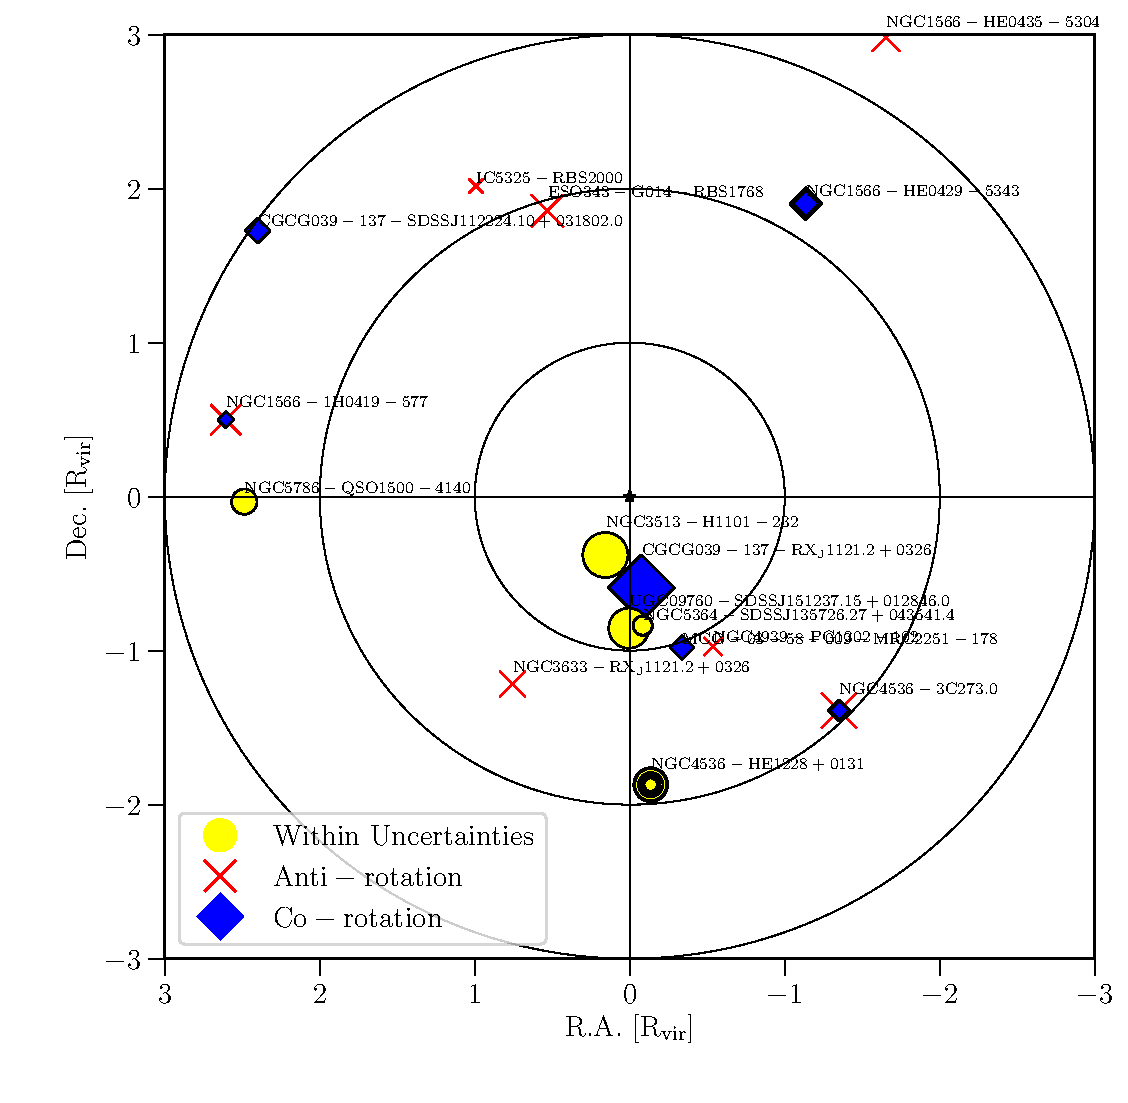
\includegraphics[width=0.60\textwidth]{SALT_map3.pdf}
        \caption{\small{A map of the locations of each absorber normalized with respect to the galaxy virial radius. Concentric rings indicate distances of 1, 2 and 3 $R_{vir}$. All galaxies are rotated to PA = 90, such that their major axis' are horizontal. The color and style of each point indicates the line-of-sight velocity compared to that of the rotation of the nearby galaxy. Blue diamonds indicate co-rotation, red X's indicate anti-rotation, and yellow circles indicate cases where either is possible due to a combination of orientation and velocity uncertainties. The size of each point is scaled to reflect the EW of the absorber. }}
%        \vspace{-5pt}
        \label{map}
\end{figure*}


%\begin{figure}[t!]
%\centering
%  \subfigure[]{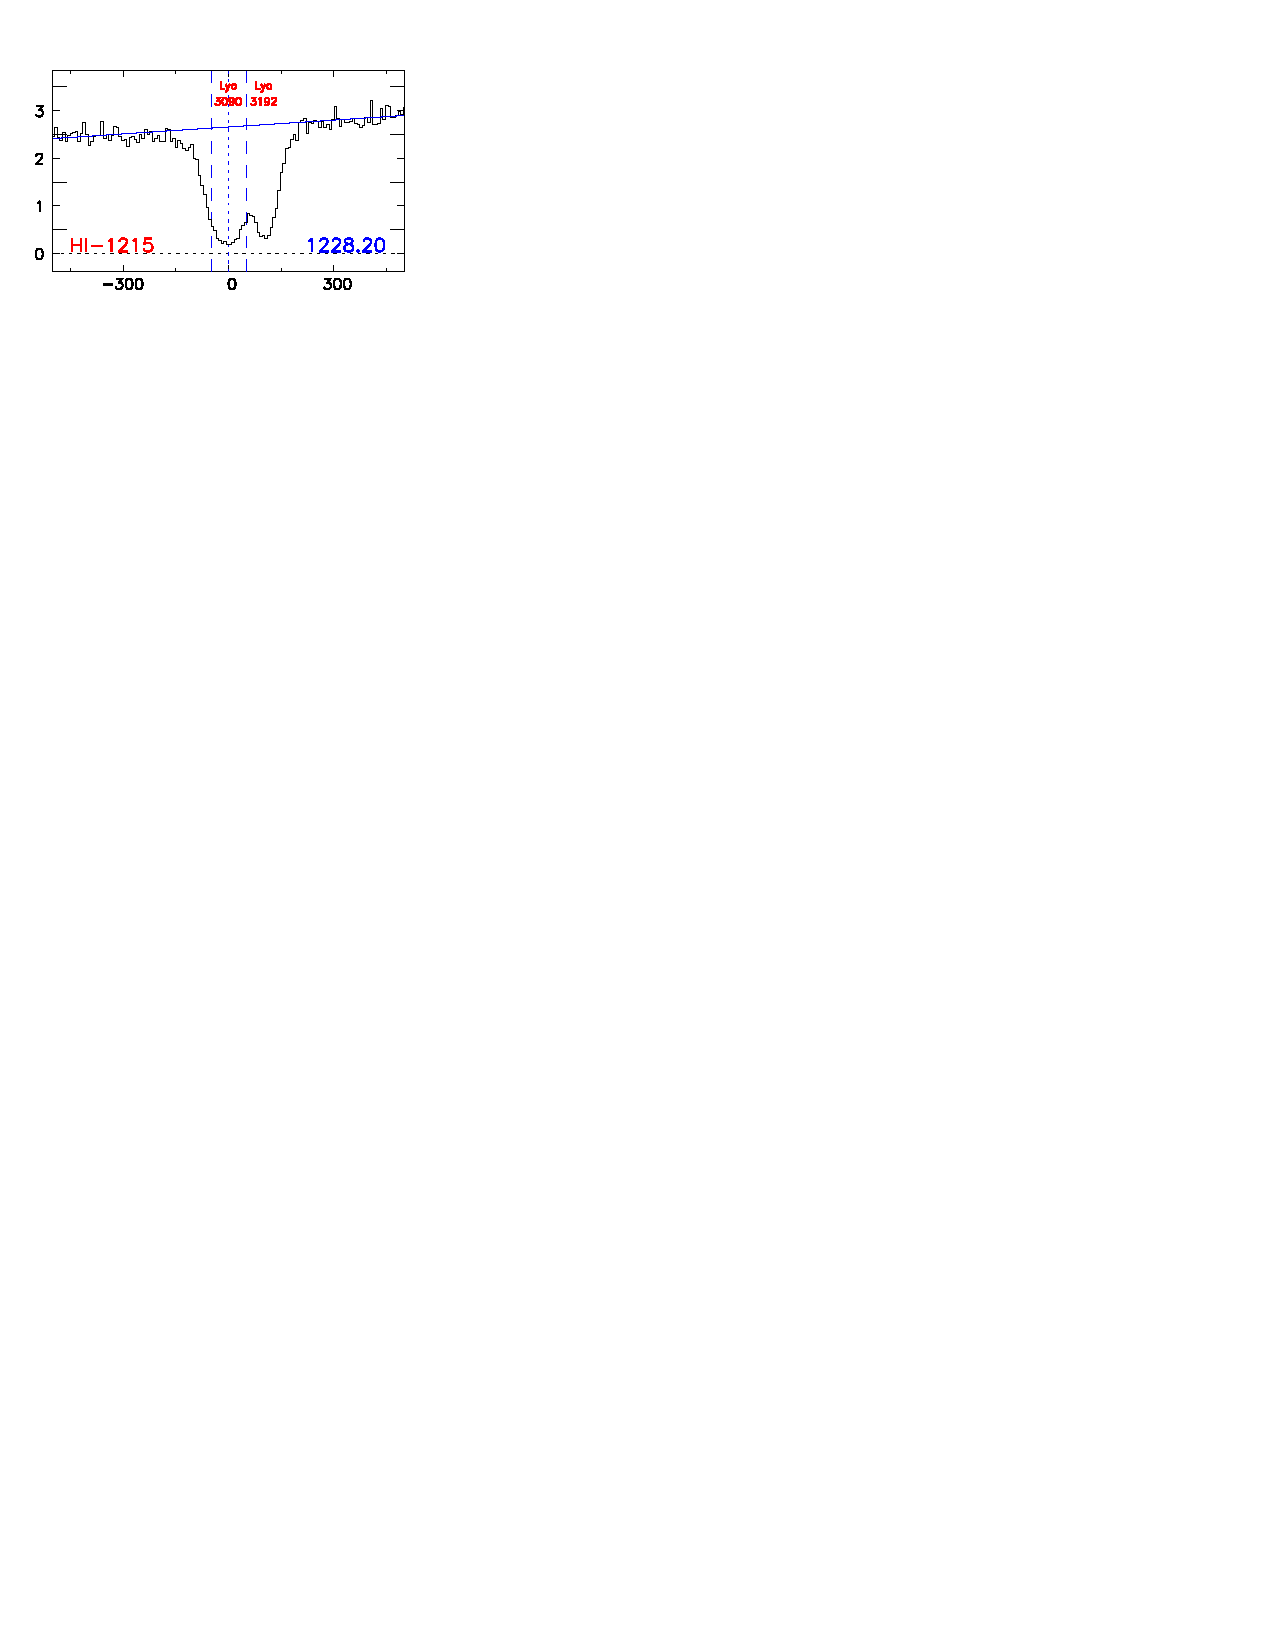
\includegraphics[width=0.87\linewidth]{fig2.pdf}}{\label{line}}
%  \subfigure[]{\includegraphics[width=1.\linewidth]{fig3.pdf}\label{impactmap}}
%  \caption{\small{a) An example of 2 Ly$\alpha$ lines found in the Mrk290 sightline at 3090 and 3192 . b) A map of \textit{all} galaxies within a 500 kpc impact parameter of target Mrk290 sightline and with velocity ($cz$) within 400 $\rm km\, s^{-1}$ of absorption detected at 3192 $\rm km\, s^{-1}$ (central black star). The galaxy NGC5987 ($v=3010$ $\rm km\, s^{-1}$, inclination = $65^{\circ}$) can be unambiguously paired with the Ly$\alpha$ absorption features at $v=3090, 3192$ $\rm km\, s^{-1}$ because it is the largest and closest galaxy in both physical and velocity space to the absorption feature.}}
%\vspace{5pt}
%\end{figure}




\section{Summary}



%\begin{table}[ht]\footnotesize
%\begin{center}
%\begin{tabular}{l l l}
% \hline \hline
% Statistic                				&  Blueshifted Absorbers   &     Redshifted Absorbers     \\ 
%  \hline \hline
% Number 	          			 		&     	22				&	26			\\
% Mean $EW$    \scriptsize $\rm [m\AA]$    &	$329 \pm 52$ 		&	$245 \pm 34$  	\\
%  
%\hline
%\end{tabular}
%\end{center}
%  \caption{\small{Average properties of the associated galaxy sample split into red and blue-shifted bins based on $\Delta v$.}}
%  \label{resultsTable}
%\end{table}


\vspace{10pt}

\indent \textbullet \indent First result


\acknowledgements

This research has made use of the NASA/IPAC Extragalactic Database (NED) which is operated by the Jet Propulsion Laboratory, California Institute of Technology, under contract with the National Aeronautics and Space Administration. Based on observations with the NASA/ESA \textit{Hubble Space Telescope}, obtained at the Space Telescope Science Institute (STScI), which is operated by the Association of Universities for Research in Astronomy, Inc., under NASA contract NAS 5-26555. \textbf{SALT ACKNOWLEDGEMENT}. Spectra were retrieved from the Barbara A. Mikulski Archive for Space Telescopes (MAST) at STScI. Over the course of this study, D.M.F. and B.P.W. were supported by grant AST-1108913, awarded by the US National Science Foundation, and by NASA grants \textit{HST}-AR-12842.01-A, \textit{HST}-AR-13893.01-A, and \textit{HST}-GO-14240 (STScI). 

\facility{HST (COS)}


\nocite{*}
\bibliography{rotation_bib}
\bibliographystyle{apj}

\end{document}
